\documentclass[18pt]{beamer} 

\usepackage{graphicx}
\usepackage[utf8]{inputenc}
\usepackage{tikz}
\usepackage{tkz-graph}
\usepackage{listings}
\usetikzlibrary{arrows}
\usetikzlibrary{shapes}

\title{Parallelising Graph Algorithms in GAP}
\author{Ivars Zubkans}
\date{April, 2014}

\begin{document}

\defverbatim[colored]\lstI{
\begin{lstlisting}[language=Ruby, mathescape]
def FW-BW(G, SCC)

  v = any vertex of G
  $FW_G(v) =$ forwards reachable vertices from v of G
  $BW_G(v) =$ backwards reachable vertices from v of G
  $S = FW_G(v) \cap BW_G(v)$
  Add S to SCC
  
  do in parallel
    FW-BW(InducedGraph($FW_G(v) \setminus S$), SCC)
    FW-BW(InducedGraph($BW_G(v) \setminus S$), SCC)
    FW-BW(InducedGraph($G \setminus (FW_G(v) \cup BW_G(v))$, SCC)
end
\end{lstlisting}
}

\frame{\titlepage}

\begin{frame}
	\frametitle{Motivation}
	
	\begin{itemize}
		\item Graphs algorithms are heavily used for modeling and solving problems
		\begin{itemize}
			\item Maze solving (BFS and DFS)
			\item Scheduling/arrangement problems (Vertex colouring)
			\item Path-finding (Dijkstra's algorithm)
		\end{itemize}
		\item GAP did not have a general purpose package for graphs
		\item Parallelism capabilities were recently added to GAP
	\end{itemize}
\end{frame}

\begin{frame}
	
	\frametitle{Graph Definition}
	
		\begin{definition}[Graph]
A $graph$  $G$ is a triple $G = (V, E, ends)$ where $V$ and $E$ are sets, while $ends$ is a function 
  \begin{equation}
  ends:E\to \mathcal P \left({V}\right)
  \end{equation}
which assigns to each element of $E$ a set of one or two elements of $V$. The elements of $V$ are called $vertices$ or $nodes$ of $G$, and elements of $E$ are called $edges$ of $G$.
\end{definition}
			
\end{frame}
	
\begin{frame}
	\frametitle{Examples}
	\framesubtitle{Undirected, Directed, Weighted }
    
	\begin{figure}[!htb]
			\minipage{0.32\textwidth}
  			\includegraphics[width=\linewidth]{fb_friends}
			\endminipage\hfill
			\minipage{0.32\textwidth}
  			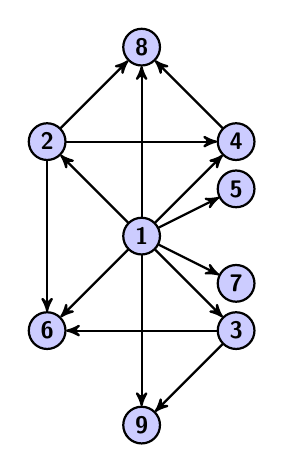
\begin{tikzpicture}[scale = 0.6,->,>=stealth',auto,
  thick,every node/.style={scale = 0.6, circle,fill=blue!20,draw,font=\sffamily\Large\bfseries}]
  \node (n2) at (-2,2) {2};
  \node (n1) at (0,0)  {1};
  \node (n5) at (2,1)  {5};
  \node (n4) at (2,2) {4};
  \node (n3) at (2,-2)  {3};
  \node (n7) at (2,-1)  {7};
  \node (n8) at (0,4)  {8};
  \node (n6) at (-2,-2)  {6};
  \node (n9) at (0,-4)  {9};

  \foreach \from/\to in {n1/n2,n1/n3,n1/n4,n1/n5,n1/n6,n1/n7,n1/n8,n1/n9, n2/n4, n2/n8, n2/n6, n3/n6, n3/n9, n4/n8}
    \draw[->] (\from) -- (\to);

\end{tikzpicture}
			\endminipage\hfill
			\minipage{0.32\textwidth}
  			\SetVertexNormal[Shape = ellipse,
                 FillColor  = blue!20,
                 LineWidth  = 2pt]
\SetUpEdge[lw         = 1.5pt,
           color      = black,
           labelcolor = white,
           labeltext  = red,
           labelstyle = {sloped,draw,text=blue, scale=0.8}]
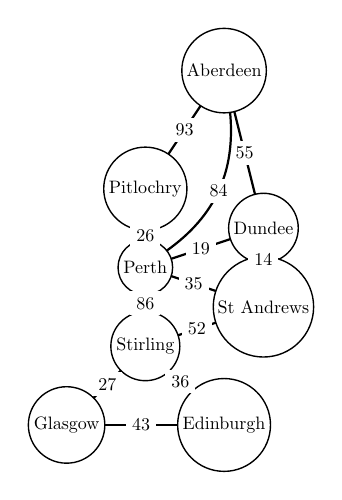
\begin{tikzpicture}[scale=0.5, every node/.style={scale = 0.65}]
   \Vertex[x=0 ,y=0]{Perth}
   \Vertex[x=0 ,y=-2]{Stirling}
   \Vertex[x=3,y=1]{Dundee}
   \Vertex[x=3 ,y=-1]{St Andrews}
   \Vertex[x=2 ,y=5]{Aberdeen}
   \Vertex[x=0 ,y=2]{Pitlochry}
   \Vertex[x=-2 ,y=-4]{Glasgow}
   \Vertex[x=2 ,y=-4]{Edinburgh}
   \Edge[label = $86$](Perth)(Stirling)
   \Edge[label = $35$](Perth)(St Andrews)
   \Edge[label = $26$](Perth)(Pitlochry)
   \Edge[label = $19$](Perth)(Dundee)
   \Edge[label = $14$](St Andrews)(Dundee)
   \Edge[label = $55$](Aberdeen)(Dundee)
   \Edge[label = $93$](Pitlochry)(Aberdeen)
   \Edge[label = $52$](St Andrews)(Stirling)
   \Edge[label = $27$](Glasgow)(Stirling)
   \Edge[label = $36$](Edinburgh)(Stirling)
   \Edge[label = $43$](Glasgow)(Edinburgh)
   \tikzset{EdgeStyle/.append style = {bend right}}
   \Edge[label = $84$](Perth)(Aberdeen)
\end{tikzpicture}
			\endminipage
		\end{figure}
\end{frame}

\begin{frame}
\frametitle{Serial and Parallel Algorithms}
	\begin{definition}[Algorithm]
		Is a step-by-step procedure for solving a problem in a finite number of steps, e.g finding finding primes.
	\end{definition}
	\begin{definition}[Serial Algorithm]
		Is an algorithm whose steps are executed in a sequence from start to finish without other computation in between.
	\end{definition}
	\begin{definition}[Parallel Algorithm]
	  Is an algorithm in which several steps are carried out simultaneously.
	\end{definition}
\end{frame}
  
  \begin{frame}
		\frametitle{Parallel Motivation and Issues}
		
		Motivation:
		 \begin{itemize}
      \item Can improve execution time for costly computations.
      \item Single core processors do not get much faster any more, the focus is on multi-core architectures.
    \end{itemize}
    
    Challenges:
    \begin{itemize}
      \item Random execution order
      \item Communication
      \item Load balancing
    \end{itemize}
  \end{frame}
  
  \begin{frame}
    \frametitle{Currently Implemented Algorithms}
    
    \begin{itemize}
      \item Parallel and serial breadth first search (BFS)
      \item Serial depth first search (DFS)
      \item Parallel and serial minimum spanning tree (MST)
      \item Serial strongly connected components (SCC)
      \item Parallel and serial vertex coloring
      \item Serial single source shortest paths.
    \end{itemize}
  \end{frame}
  
  \begin{frame}
    \frametitle{Strongly Connected components}
    
    \begin{definition}[Strongly connected component]
    Let $G=(V, E, ends)$ be directed graph, then a strongly connected component (SCC) of $G$ is a maximal set of vertices $C\subset V$, such that for all $u,v \in C$, there is a path from $u$ to $v$  and vice versa.
    \end{definition}
    
\SetVertexNormal[Shape      = circle,
                 FillColor  = blue!20,
                 LineWidth  = 2pt]
\SetUpEdge[lw         = 3pt,
           color      = black,
           labelcolor = white,
           labeltext  = red,
           labelstyle = {sloped,draw,text=blue}]
\begin{center}
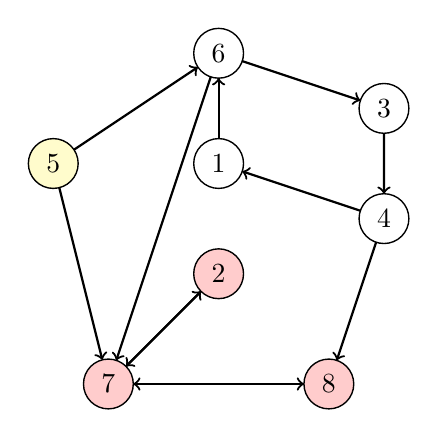
\begin{tikzpicture}[scale = 0.7]
   \tikzset{EdgeStyle/.style={->}}
   \Vertex[x=0 ,y=0]{1}
   \Vertex[x=3,y=1]{3}
   \Vertex[x=3 ,y=-1]{4}
   \Vertex[x=0 ,y=2]{6}
   \tikzset{VertexStyle/.append  style={fill=red!20}}
   \Vertex[x=0 ,y=-2]{2}
   \Vertex[x=-2 ,y=-4]{7}
   \Vertex[x=2 ,y=-4]{8}
   \tikzset{VertexStyle/.append  style={fill=yellow!20}}
   \Vertex[x=-3 ,y=0]{5}
   \Edge(6)(3)
   \Edge(3)(4)
   \Edge(4)(1)
   \Edge(1)(6)
   \Edge(4)(8)
   \Edge(6)(7)
   \Edge(2)(7)
   \Edge(7)(2)
   \Edge(7)(8)
   \Edge(8)(7)
   \Edge(5)(6)
   \Edge(5)(7)
\end{tikzpicture}
\end{center}    
    
  \end{frame}
  
  \begin{frame}
  \frametitle{Tarjan's Serial SCC Algorithm}
  
    \begin{itemize}
      \item based on depth first search (DFS).
      \item indexes vertices as they are traversed by DFS
      \item when returning from recursive DFS, every vertex gets a reachable vertex with the least index as its SCC representive.
    \end{itemize}  
  \end{frame}  
  
  \begin{frame}
    \frametitle{Forwards-Backwards Parallel SCC Algorithm}
      
    %The classic sequential method for SCC detection is difficult to parallelise, but an algorithm that is much better suited for parallelisation, called Forward-Backward (FW-BW) has been devised.
    
    \lstI
    
  \end{frame}
  
  \begin{frame}
    \frametitle{FW-BW Base Theorem}
    
    Let $G=(V, E, ends)$ be a directed graph and v be vertex in G. Then $FW_G(v) \cap BW_G(v)$ is a unique SCC in G. Furthermore, every other SCC in G is either a subset of $FW_G(v) \setminus BW_G(v)$ or $BW_G(v) \setminus FW_G(v)$, or  $Rem_G(v)=V \setminus (FW_G(v) \cup BW_G(v))$
  \end{frame}
  
   \begin{frame}
    \frametitle{SCC parallel example}
    
    \begin{figure}[!htb]
			\minipage{0.32\textwidth}
  			\SetVertexNormal[Shape      = circle,
                 FillColor  = blue!20,
                 LineWidth  = 2pt]
\SetUpEdge[lw         = 3pt,
           color      = black,
           labelcolor = white,
           labeltext  = red,
           labelstyle = {sloped,draw,text=blue}]
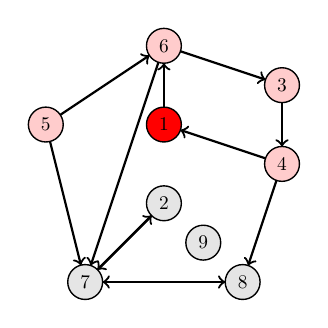
\begin{tikzpicture}[scale = 0.5]
   \tikzset{EdgeStyle/.style={->}}
   \tikzset{VertexStyle/.append  style={fill=red, scale = 0.7}}
   \Vertex[x=0 ,y=0]{1}
   \tikzset{VertexStyle/.append  style={fill=red!20}}
   \Vertex[x=3,y=1]{3}
   \Vertex[x=3 ,y=-1]{4}
   \Vertex[x=0 ,y=2]{6}
   \tikzset{VertexStyle/.append  style={fill=gray!20}}
   \Vertex[x=0 ,y=-2]{2}
   \Vertex[x=-2 ,y=-4]{7}
   \Vertex[x=2 ,y=-4]{8}
   \tikzset{VertexStyle/.append  style={fill=red!20}}
   \Vertex[x=-3 ,y=0]{5}
   \tikzset{VertexStyle/.append  style={fill=gray!20}}
   \Vertex[x=1 ,y=-3]{9}
   \Edge(6)(3)
   \Edge(3)(4)
   \Edge(4)(1)
   \Edge(1)(6)
   \Edge(4)(8)
   \Edge(6)(7)
   \Edge(2)(7)
   \Edge(7)(2)
   \Edge(7)(8)
   \Edge(8)(7)
   \Edge(5)(6)
   \Edge(5)(7)
\end{tikzpicture}
\center{Backwards reachable}
			\endminipage\hfill
			\minipage{0.32\textwidth}
  			\SetVertexNormal[Shape      = circle,
                 FillColor  = blue!20,
                 LineWidth  = 2pt]
\SetUpEdge[lw         = 3pt,
           color      = black,
           labelcolor = white,
           labeltext  = red,
           labelstyle = {sloped,draw,text=blue}]
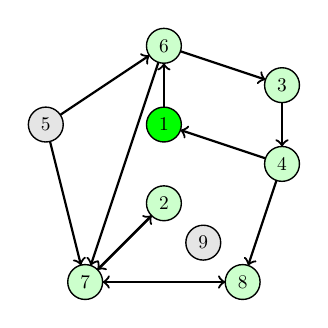
\begin{tikzpicture}[scale=0.5]
   \tikzset{EdgeStyle/.style={->}}
   \tikzset{VertexStyle/.append  style={fill=green, scale=0.7]}}
   \Vertex[x=0 ,y=0]{1}
   \tikzset{VertexStyle/.append  style={fill=green!20}}
   \Vertex[x=3,y=1]{3}
   \Vertex[x=3 ,y=-1]{4}
   \Vertex[x=0 ,y=2]{6}
   \tikzset{VertexStyle/.append  style={fill=green!20}}
   \Vertex[x=0 ,y=-2]{2}
   \Vertex[x=-2 ,y=-4]{7}
   \Vertex[x=2 ,y=-4]{8}
   \tikzset{VertexStyle/.append  style={fill=gray!20}}
   \Vertex[x=-3 ,y=0]{5}
   \tikzset{VertexStyle/.append  style={fill=gray!20}}
   \Vertex[x=1 ,y=-3]{9}
   \Edge(6)(3)
   \Edge(3)(4)
   \Edge(4)(1)
   \Edge(1)(6)
   \Edge(4)(8)
   \Edge(6)(7)
   \Edge(2)(7)
   \Edge(7)(2)
   \Edge(7)(8)
   \Edge(8)(7)
   \Edge(5)(6)
   \Edge(5)(7)
\end{tikzpicture}
\center{Forwards reachable}
			\endminipage\hfill
			\minipage{0.32\textwidth}
  			\SetVertexNormal[Shape      = circle,
                 FillColor  = blue!20,
                 LineWidth  = 2pt]
\SetUpEdge[lw         = 3pt,
           color      = black,
           labelcolor = white,
           labeltext  = red,
           labelstyle = {sloped,draw,text=blue}]
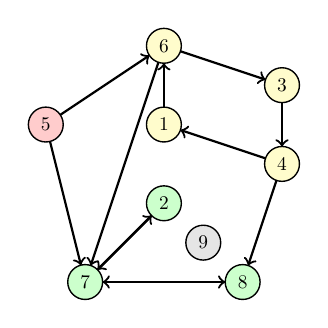
\begin{tikzpicture}[scale=0.5]
   \tikzset{EdgeStyle/.style={->}}
   \tikzset{VertexStyle/.append  style={fill=yellow!20, scale=0.7]}}
   \Vertex[x=0 ,y=0]{1}
   \tikzset{VertexStyle/.append  style={fill=yellow!20}}
   \Vertex[x=3,y=1]{3}
   \Vertex[x=3 ,y=-1]{4}
   \Vertex[x=0 ,y=2]{6}
   \tikzset{VertexStyle/.append  style={fill=green!20}}
   \Vertex[x=0 ,y=-2]{2}
   \Vertex[x=-2 ,y=-4]{7}
   \Vertex[x=2 ,y=-4]{8}
   \tikzset{VertexStyle/.append  style={fill=red!20}}
   \Vertex[x=-3 ,y=0]{5}
   \tikzset{VertexStyle/.append  style={fill=gray!20}}
   \Vertex[x=1 ,y=-3]{9}
   \Edge(6)(3)
   \Edge(3)(4)
   \Edge(4)(1)
   \Edge(1)(6)
   \Edge(4)(8)
   \Edge(6)(7)
   \Edge(2)(7)
   \Edge(7)(2)
   \Edge(7)(8)
   \Edge(8)(7)
   \Edge(5)(6)
   \Edge(5)(7)
\end{tikzpicture}
\center{Disjoint parts}
			\endminipage\hfill
		\end{figure}
  \end{frame}
  
    \begin{frame}
    \frametitle{MST experimental results}
    
    \begin{center}
      \includegraphics[scale = 0.35]{MSTPlot}
    \end{center}
  \end{frame}
  
  \begin{frame}
    \frametitle{MST experimental results}
    
    \begin{center}
      \includegraphics[scale = 0.45]{MSTPlot2}
    \end{center}
    
  \end{frame}
  
  \begin{frame}
    \frametitle{Conclusions}
    
    \begin{itemize}
    	\item Parallel algorithms can be faster
    	\item Add complexity
    	\item Introduce overhead
    	\item Use mathematical properties to partition the problem
    \end{itemize}
    
  \end{frame}
\end{document}